%%%%%%%%%%%%%%%%%%%%%%%%%%%%%%%%%%%
%%%  Filename: thesis_template.tex
%%%  ---
%%%  Template for Master Thesis at DTETI UGM   		
%%%  Created using thesisdtetiugm.cls
%%%  --- 
%%%  Written by Canggih Puspo Wibowo
%%%  [canggihpw@gmail.com]
%%%%%%%%%%%%%%%%%%%%%%%%%%%%%%%%%%%

%% Use option "bahasa" or "english" 
%%    to change the basic language used
%% User option "bachelor", "master", or "doctoral"
%% 	  to change the degree
% \documentclass[<bachelor/master/doctoral>,<bahasa/english>]{thesisdtetiugm}
\documentclass[bachelor,bahasa]{thesisdtetiugm}
%======================================
% Information Input
%======================================
% Input author's name and ID number
\author{DHIAS MUHAMMAD NAUFAL}{19/446774/TK/49879}
% Input the thesis' title
\title{DESAIN GAMIFIKASI UNTUK APLIKASI PEMBELAJARAN \emph{CLINICAL DECISION SUPPORT SYSTEM (CDSS)}}
% Program and the head of the program
\program{TEKNOLOGI INFORMASI}{<<Program coordinator>>}{<<NIP>>}
% Name of department head and NIP
\departmenthead{<<Head of the department>>}{<<NIP>>}
\major{<<Major>>}
\yearsubmit{2023}
\examdate{28 Juni}
% Name of thesis supervisors/promotors
\addsupervisor{Adhistya Erna Permanasari, S.T., M.T., Ph.D.}{NIP 198104292008122001}
\addsupervisor{Prof. Ir. Paulus Insap Santosa, M.Sc., Ph.D., IPU.}{NIP 196101081985031002}
%\addsupervisor{<<Supervisor 3>>}{<<NIP>>}
% Name of examiners
%\addexaminer{<<Examiner 1>>}{<<NIP 1>>}
%\addexaminer{<<Examiner 2>>}{<<NIP 2>>}
%\addexaminer{<<Examiner 3>>}{<<NIP 3>>}
%\addexaminer{<<Examiner 4>>}{<<NIP 4>>}
%\addexaminer{<<Examiner 5>>}{<<NIP 5>>}
%\addexaminer{<<Examiner 6>>}{<<NIP 6>>}
%\addexaminer{<<Examiner 7>>}{<<NIP 7>>}
%\addexaminer{<<Examiner 8>>}{<<NIP 8>>}
%\addexaminer{<<Examiner 9>>}{<<NIP 9>>}

%======================================
% correct bad hyphenation here [example]
% \babelhyphenation[<<english/bahasa>>]{op-tical net-works semi-conduc-tor}
%% Uncomment block of code below to disable hyphenation
%\tolerance=1
%\emergencystretch=\maxdimen
%\hyphenpenalty=10000
%\hbadness=10000

\begin{document}
%======================================
% Create cover etc
%======================================

%---- COVER ----
%\printcover{sample/logougm.png}{Pendadaran/Tesis/Ringkasan Tesis*}
\printcover{sample/logougm.png}{Bachelor}
% *Choose one

%---- ENDORSEMENT PAGE ----
% Select endorsement page type. If you want to use your own PDF file,  
% 	use \printendorsementpdf, or if you want to use JPG file, use 
% 	\printendorsementjpg. Otherwise, use \printendorsement.
% 	Choose one only. Comment out unused command(s).
%
\printendorsement
%\printendorsementpdf
%\printendorsementjpg{sample/scanned-endorsement.jpg}

%---- DEDICATION PAGE ----
\chapterstatement{contents/statement/statement}
%\chapterstatementjpg{sample/scanned-statement.jpg}

\chapterdedication{contents/dedication/dedication}

%---- STATEMENT PAGE ----
% Select statement page type. If you want to use your own JPG file,  
%	use \chapterstatementjpg{<your *.jpg file path>}. Otherwise, 
%	use \chapterstatement{contents/statement/statement}.
%	Choose one only. Comment out unused command(s).
%


%---- PREFACE PAGE ----
\chapterpreface{contents/preface/preface}

%======================================
% Create Table of Contents, List of Figures, List of Tables
% <Do not change this part>
%======================================
\thetoc
\onehalfspacing
\tableofcontents
\singlespacing
\thelot
\listoftables
\thelof
\listoffigures

%======================================

%---- NOMENCLATURE PAGE ----
\chapternomenclature{contents/nomenclature/nomenclature}

%---- INTISARI PAGE----
\chapterintisari{contents/abstract/intisari}

%---- ABSTRACT PAGE----
\chapterabstract{contents/abstract/abstract}


%======================================



%======================================
%  MAIN TEXT
%======================================
\startmain
% You can change 
%    the filename and location of the files inputted
\chapter{Pendahuluan}
Pada bab pendahuluan ini akan dipaparkan mengenai Latar Belakang, Rumusan Masalah, dan Batasan Masalah dalam menentukan pengerjaan Tugas Akhir.
Kemudian dijelaskan juga mengenai Tujuan dari dibuatnya tugas akhir ini, dan Manfaat yang akan diperoleh dari hasil akhir.
Setelah itu, di akhir bab ini akan dijelaskan mengenai sistematika penulisan sebagai gambaran umum mengenai isi dari tugas akhir ini.

\section{Latar Belakang}
%========= Paragraf 1 : Pembahasan CDSS sebagai Subject Media Pembelajaran yang akan dibuat=======================
Sistem Diagnosis berbasis Pendukung Keputusan (SDBPK) atau yang lebih dikenal dengan \textit{Clinical Decision Supoort System (CDSS)}
merupakan sistem komputer yang dibuat spesifik untuk membantu tenaga kesahatan.
Sistem ini merupakan sebuah terobosan dalam dunia medis yang dapat meningkatkan kualitas perawatan medis dalam pengambilan keputusan.
Sistem ini penting untuk dipelajari

Untuk meningkatkan kesadaran akan adanya sistem ini, 
Importance of CDSS to Public

Teknologi Informasi mengalami perkembangan yang sangat pesat, berbanding lurus dengan beragamnya pemanfaatan Teknologi Informasi dalam konteks penyampaian informasi.
Salah satunya ialah hadirnya media pembelajaran yang mengadopsi Teknologi Informasi untuk mempermudah manusia dalam penyampaian informasi pembelajaran.
Media pembelajaran sendiri adalah sebuah medium yang memuat informasi atau pesan instruksional dan dapat digunakan dala proses pembelajaran.
Media pembelajaran merupakan elemen yang cukup penting bagi peserta didik untuk membantu memperoleh konsep baru, keterampilan dan kompetensi.
Dengan memanfaatkan Media pembelajaran yang tepat, akan membantu peserta didik untuk meningkatkan interaksi dalam proses pembelajaran 
sehingga peserta didik tidak akan merasa bosan dalam pembelajaran\cite{hasan2021media}.

Media pembelajaran yang mengadopsi Teknologi informasi dikenal juga dengan E-Learning, sekarang sudah ada M-Learning dimana M-learning dibandingkan E-Learning baisa blablabla

Goals dari masalah yang dihadapi ialah membuat suatu media pembelajaran yang tidak monoton dan lebih menarik (dapat meningkatkan motvasi).
Gamifikasi merupakan metode blablabala
% menjanjikan akan meningkatnya kualitas perawatan klinis dengan membantu tenaga medis
% untuk mengakses dan menerapkan pengetahuan klinis secara relevan dan efisien, dengan demikian dapat mengambil keputusan yang lebih baik
% sesuai dengan perkembangan terbaru dalam bidang medis.


% Tidak semua orang mengetahui seberapa kuat sistem ini akan membantu kita untuk mengambil sebuah keputusan medis.


% Sistem tersebut dipelajari secara khusus pada program studi Teknik Biomedis Departemen Teknik Elektro dan Teknologi Informasi (DTETI) Universitas Gadjah Mada.
% %========= Ngejelasin akar Masalah ==========
% Berdasarkan hasil wawancara yang dilakukan dengan mahasiswa Teknik Biomedis yang sudah pernah mengambil mata kuliah tersebut, 
% mereka menyampaikan bahwa mereka mengalami kesulitan dalam memahami inti dari mata kuliah tersebut.
% Selain karena mata kuliah ini tergolong baru, 
% Faktor kesulitan tersebut tidak hanya disebabkan oleh sifat baru mata kuliah ini, 
% tetapi juga karena adanya dua core materi yang dianggap kompleks. 
% Core materi pertama adalah pengetahuan tentang Sistem Pembantu Keputusan (SPK) yang dipelajari oleh mahasiswa Teknologi Informasi, 
% sedangkan core materi kedua adalah pengetahuan tentang Diagnosis yang dipelajari oleh mahasiswa dari Kluster Kesehatan.
% Karena kompleksitas materi yang perlu dipahami, metode penyampaian yang efektif merupakan kunci dalam proses pembelajaran.

% Pendidikan merupakan salah satu aspek dalam kehidupan manusia yang memainkan peran penting dalam mengembangkan sebuah individu dan masyarakat.
% Melalui pendidikan, Individu akan memperoleh pengetahuan, keterampilan dan nilai-nilai positif.
% Nilai-nilai tersebut dapat diperoleh melalui sebuah proses pembelajaran yang dilakukan oleh seorang individu.
% Proses Pembelajaran dapat melibatkan dua pihak yaitu siswa sebagai pebelajar dan guru sebagai fasilitator, yang terpenting dalam kegiatan pembelajaran adalah terjadinya proses belajar \textit{(Learning Process)}.
% Salah satu elemen penting dalam sebuauh proses pembelajaran ialah adanya media yang menjadi sarana penyampaian informasi yang dilakukan antar
% Namun, dalam proses pelaksanaannya sering kali siswa atau mahasiswa mengalami kesulitan dalam mempertahankan motivasi dan minat dalam proses pembelajaran.
% Salah satu faktor yang memicu masalah tersebut ialah kurangnya ketertarikan dan keterlibatan mahasiswa terhadap materi yang disajikan dengan cara konvensional.
% Cara konvensional yang dimaksud merupakan pembelajaran yang berpusat pada guru, dimana guru berperan dalam mengendalikan penyajian pembelajaran.
% Cara ini juga diyakini masih belum efektif dikarenakan memerlukan kehadiran dua pihak dalam pelaksanaanya.
% Murid tidak dapat ikut andil atau pasif dalam proses penmbelajarannya kecuali kedua belah pihak bertemu pada sebuah pertemuan.

% %========== Paragraf 2 : Pembahasan adopsi teknologi pada Pendidikan =================== kata kunci %Perkembangan Teknologi -> Dibutuhkan media pembalajaran yang menarik
% Pengadopsian Teknologi Informasi merupakan salah satu upaya untuk mengatasi tantangan dalam pembelajaran konvensional tersebut.
% Salah satu solusi yang menarik ialah penggunakan teknologi e-learning atau pembelajaran elektronik.
% E-learning sendiri merupakan sebuah metode pendekatan pembelajaran dengan mengadopsi Teknolog Informasi dalam prosesnya, khususnya internet, sebagai media utama untuk menyampaikan materi pembelajaran kepada siswa atau mahasiswa. 


% Penerapan e-learning memberikan banyak manfaat untuk proses pembelajaran.
% Dengan penerapan teknologi ini, siswa atau mahasiswa akan memiliki fleksibilitas dalam mengatur waktu dan tempat belajar.
% Mereka dapat mengakses materi pembelajaran di mana saja dan kapan saja selama terhubung ke internet.
% Hal ini tergolong lebih efektif karena memungkinkan adanya pembelajaran jarak jauh, mengatasi keterbatasan geografis dan jadwal yang kaku.
% Selain itu, e-learning dapat meningkatkan kemungkinan interaksi yang lebih aktif antara siswa atau mahasiswa dengan materi pembelajaran.
% Melalui fitur-fitur seperti forum diskusi, kuis online, dan tugas daring, siswa atau mahasiswa dapat berpartisipasi secara aktif dalam proses pembelajaran.

% Meskipun e-learing telah memberikan solusi dalam hal fleksibilitas dan efektivitas interaksi, masih ada tantangan dalam mempertahankan motivasi dan keterlibatan siswa atau mahasiswa.
% Dalam hal ini, penerapan desain gamifikasi pada sebuah media pembelajaran dapat menjadi salah satu solusi yang diyakini efektif untuk meningkatkan motivasi dan keterlibatkan siswa atau mahasiswa.
% Gamifikasi merupakan sebuah pendekatan yang mengadaptasi elemen-elemen permainan atau game design dalam konteks non-permainan untuk meningkatkan motivasi dan partisipasi siswa atau mahasiswa. 

Dalam penelitian ini, penulis akan membahas proses pengembangan desain gamifikasi pada sebuah media pembelajaran elektronik yang akan dikembangkan.
Dengan menggunakan elemen-elemen seperti pemberian poin, tingkat, pencapaian, kompetisi, dan hadiah dalam aplikasi pembelajaran e-learning, diharapkan pendekatan ini dapat memicu minat, antusiasme, dan keterlibatan siswa atau mahasiswa.


\section{Rumusan Masalah}
Berdasarkan pemaparan pada bagian latar belakang, maka dapat dirumuskan masalah sebagai berikut :
\begin{enumerate}
	\item Proses pembelajaran pada Mata Kuliah SDBPK masih belum optimal dikarenakan merupakan sebuah mata kuliah yang baru dan cukup kompleks
	\item Mata Kuliah SDBPK di Departemen Teknik Elektro dan Teknologi Informasi (DTETI) belum memiliki media pembelajaran yang cocok untuk mahasiswanya
\end{enumerate}

%-------------------------------------------------	

\section{Tujuan Penelitian}

Tujuan dari pengembangan tugas akhir ini ialah :
\begin{enumerate}
	\item Mengembangkan media pembelajaran untuk mata kuliah Sistem Diagnosis Berbasis Pembantu Keputusan\textit{(SDBPK)} dengan adaptasi Gamifikasi untuk menciptakan media pembelajaran yang interaktif dan menarik
	\item Menguji fungsionalitas, kegunaan, dan pengalaman pengguna dari aplikasi pembelajaran kepada calon penggunanya.
\end{enumerate}
% \newpage 	
% \vspace{5mm}
% \begin{minipage}{0.92\textwidth}
% Berikut adalah beberapa contoh tujuan penelitian yang sesuai dengan topik 
% “perbaikan efisiensi penghematan energi pada sistem pencahayaan rumah tangga 
% melalui implementasi teknologi kontrol otomatis”:
% \end{minipage}
\section{Batasan Penelitian}
Berdasarkan keterbatasan waktu pengembangan dan sumber daya manusia, pembahasan yang terdapat pada Tugas Akhir ini memiliki beberapa batasan, diantaranya ialah :
\begin{enumerate}
\item Objek penelitian: spesifikasikan objek penelitian dan bidang teknik yang diteliti, misalnya teknik elektro, teknik biomedis, atau teknologi informasi.
% \item Objek Penelitian: Analisis perbandingan efektivitas dan efisiensi antara sistem manajemen proyek tradisional dan sistem manajemen proyek berbasis teknologi informasi. 
\item Metode penelitian: jelaskan metode penelitian yang akan digunakan dan 
bagaimana itu membatasi area penelitian, misalnya metode eksperimental, 
analisis simulasi, dll.
% \item Metode Penelitian: Penelitian kualitatif dengan menggunakan wawancara dan 
% survei terhadap para pelaku proyek di berbagai perusahaan. 
\item Waktu dan tempat penelitian: batasi waktu dan tempat penelitian, 
misalnya studi kasus pada tahun tertentu atau wilayah tertentu.
% \item Waktu dan Tempat Penelitian: Waktu penelitian adalah Januari-Juni 2022 di 
% perusahaan-perusahaan di wilayah Bantul. 
\item Populasi dan sampel: jelaskan populasi dan sampel yang akan diteliti, misalnya produk, mesin, atau sistem.
% \item Populasi dan Sampel: Populasi nya adalah perusahaan yang melakukan proyek, dan sampel diambil sebanyak 10 perusahaan yang menerapkan sistem manajemen 
% proyek tradisional dan 10 perusahaan yang menggunakan sistem manajemen 
% proyek berbasis teknologi informasi. 
\item Variabel dan hipotesis: jelaskan variabel yang akan diteliti dan hipotesis yang akan dibuktikan atau ditolak.
% \item Hipotesis: bahwa sistem manajemen proyek berbasis teknologi informasi lebih efektif dan efisien dibandingkan dengan sistem manajemen proyek tradisional.
\item Keterbatasan Penelitian: Keterbatasan penelitian adalah hambatan yang muncul dalam proses penelitian, seperti sumber daya yang terbatas, waktu, metodologi, dan kemampuan peneliti, yang mempengaruhi hasil dan validitas dari hasil penelitian.
% \item Keterbatasan Penelitian: Keterbatasan penelitian adalah penelitian hanya dilakukan pada perusahaan di wilayah Bantul dan hanya melibatkan wawancara dan survei sebagai metode pengumpulan data.
\end{enumerate}

\section{Manfaat Penelitian}
Dengan dikembangkannya Tugas Akhir ini diharapakan akan membawa manfaat kepada Mahasiswa DTETI

\begin{enumerate}
	\item Diaharapkan dengan dikembangkannya aplikasi ini dapat bermanfaat dalam kegiatan belajar mengajar Mahasiswa Departemen Teknik Elektro dan Teknologi Informasi 
	\item Diharapkan juga Tugas Akhir ini menjadi sebuah media pembelajaran yang dapat meningkatkan motivasi dalam pembelajaran
\end{enumerate}

\section{Sistematika Penulisan}
\begin{enumerate}
	\item Bab I Mengurai dan menjelaskan tentang latar belakang, rumusan 
	masalah yang akan dijawab pada penelitian ini, batasan masalah yang membatasi 
	pelaksanaan dari penelitian ini, tujuan yang akan dicapai pada penelitian ini, serta manfaat 
	penelitian bagi pihak-pihak terkait.
	
	\item Bab II berisi tentang metodologi penelitian yang terdiri dari desain penelitian, sumber data, Teknik pengumpulan data dan Teknik analisis data.
	\item BAB III berisi
	\item BAB IV berisi
	\item BAB V berisi
\end{enumerate}


\chapter{Tinjauan Pustaka dan Dasar Teori}
Bab ini akan membahas tinjauan pustaka yang mencakup penelitian-penelitian sebelumnya sebagai referensi untuk melaksanakan tugas akhir. Selain itu, akan dijelaskan tentang teori-teori yang menjadi dasar dalam pembuatan aplikasi tugas akhir.
\section{Tinjauan Pustaka}
% ================================= Penelitian Designing Gamification for Programming Learning Applications =================================
Gamifikasi telah terbukti menjadi strategi yang efektif dalam meningkatkan minat dan motivasi belajar. 
Berdasarkan beberapa studi yang ada, pengimplementasian gamifikasi yang tepat akan meningkatkan ketertarikan dan motivasi murid dalam proses pembelajaran \cite{EnjoyLearningLikeGaming}.
Salah satu studi yang dilakukan pada tahun 2022 oleh Evan Pradanika, Yani Widyani, dan Yanti Rusmawati dengan judul \textit{Designing Gamification for Programming Learning Applications } \cite{GamificationInProgLang} membahas mengenai penerapan gamifikasi
dalam sebuah pembelajaran pemrograman. Studi tersebut menerangkan sebuah perancangan desain sistem menggunakan pendekatan \textit{Activity-centered Design} dimana perancangan ini berfokus pada aktivitas utama pembelajaran\cite{GamificationInProgLang}. 
Implementasi gamifikasi pada penelitian ini berpedoman pada hubungan antara jenis-jenis pengetahuan atau \textit{Type of Knowledge} yang memiliki elemen gamifiaksinya masing masing.
Hubungan ini dijelaskan dalam buku yang ditulis oleh Karl M. Kapp yang berjudul \textit{"The Gamification of Learning and Instruction : Game-based method and strategies for training and education"}\cite{kapp2012gamification}.
Proses pengembangan desain gamifikasi dalam penelitian ini didasari dengan kategori pembelajarannya sendiri yaitu ilmu pemrograman yang dikategorikan sebagai \textit{declarative knowledge}.
Dengan mengevaluasi aplikasi pembelajaran pemrograman yang sudah ada di pasaran, Evan Pradanika dan teman-temannya merumuskan desain tersebut berdasarkan kebutuhan user, dan aktivitas pemrogramannya sendiri.
Sehingga, elemeng gamifikasi yang digunakan dalam penelitian ini adalah
\textit{Trivia} yang diterapkan dalam latihan-latihan dalam bentuk jawaban singkat dan pilihan ganda,
\textit{Matching} diterapkan dalam latihan-latihan dalam bentuk seret dan lepas,
\textit{Challenges} diterapkan dalam bentuk prestasi yang dapat diperoleh oleh pengguna.
Keluaran dari penelitian ini ialah sebuah \textit{High-fidelity prototype} (gambar \ref*{fig:High-fidelity prototype Evan}) dari aplikasi pembelajaran pemrograman yang sudah dirumuskan.
Kemudian desain tersebut diujikan dan dievaluasi menggunakan \textit{Usability Testing dan User Experience Goals} untuk mengukur perfroma interaktif produk terhadap penggunanya.
Usability teting yang dilakukan berupa \textit{Completion Rate} untuk mengukur efektivitas, \textit{System Usability Scale (SUS)} untuk mengukur kebergunaan,
\textit{Single Ease Question (SEQ)} untuk mengukur tingkat kesulitan dari aktivitas yang diberikan, \textit{Intrinsic Motivation Inventory (IMI)} yang merupakan instrumentasi untuk mengukur motivasi,
dan \textit{User Engagement Scale-Short Form (UES-SF)} untuk mengukur keterlibatan.
% Untuk konteks pembelajaran pemrograman, pemrograman senriri dapat dikategorikan sebagai pengetahuan deklaratif karena memungkinkan pembuatan variabel dengan tipe yang telah ditentukan oleh bahasa pemrograman. 
% Selain itu, pemrograman juga termasuk ke dalam pengetahuan prosedural karena melibatkan urutan eksekusi instruksi dalam sebuah program. 
% Selanjutnya, pemrograman juga termasuk pengetahuan konseptual karena memiliki beberapa konstruksi yang dapat digunakan, seperti if-then-else dan loop, yang merupakan konsep asli dari bahasa pemrograman itu sendiri.
% \newpage
%  \begin{table}[H]
% 	\caption{Domain Pembelajaran dan Teknik Pembelajaran dan Gamifikasi Terkait \cite{kapp2012gamification}}
% 	\vspace{0.5em}
% 	\centering
% 	\begin{tabular}{|m{5cm}|m{5cm}|m{4cm}|}
% 		\hline
%         \multicolumn{1}{|c|}{\textbf{Type of Knowledge}} & \multicolumn{1}{c|}{\textbf{Gamification Elements}} & \multicolumn{1}{c|}{\textbf{Examples}} \\ 
% 		\hline 
%         \hline
% 		Declarative Knowledge & Stories/Narrative, Sorting, Matching, Replayability & Trivia, Hangman, Drag and Drop \\\hline
% 		Conceptual Knowledge & Matching and sorting, Experiencing the concept  & Wack a Mole, You Bet! \\\hline
% 		Rules-Based Knowledge  & Experience Consequences  & Board games, Simulated work tasks \\ \hline
%         Procedural Knowledge  & Software challenges, Practice & Data Miner, Software scenarios \\\hline
%         Soft Skills & Social Simulator  & Leadership simulation  \\\hline
%         Affective Knowledge & Immersion, Providing success, Encouragement from a celebrity-type figures  & Darfur Is Dying  \\\hline
%         Psychomotor Domain & Demonstration, Haptic devices  & Virtual Surgery Simulator  \\
%         \hline
% 	\end{tabular}
% 	\label{Tab: Tabel Type of Knowledge and Gamification}
% \end{table}
\newpage
\begin{figure}[htbp]
	\centering
	\begin{subfigure}[b]{0.4\textwidth}
		\centering
	  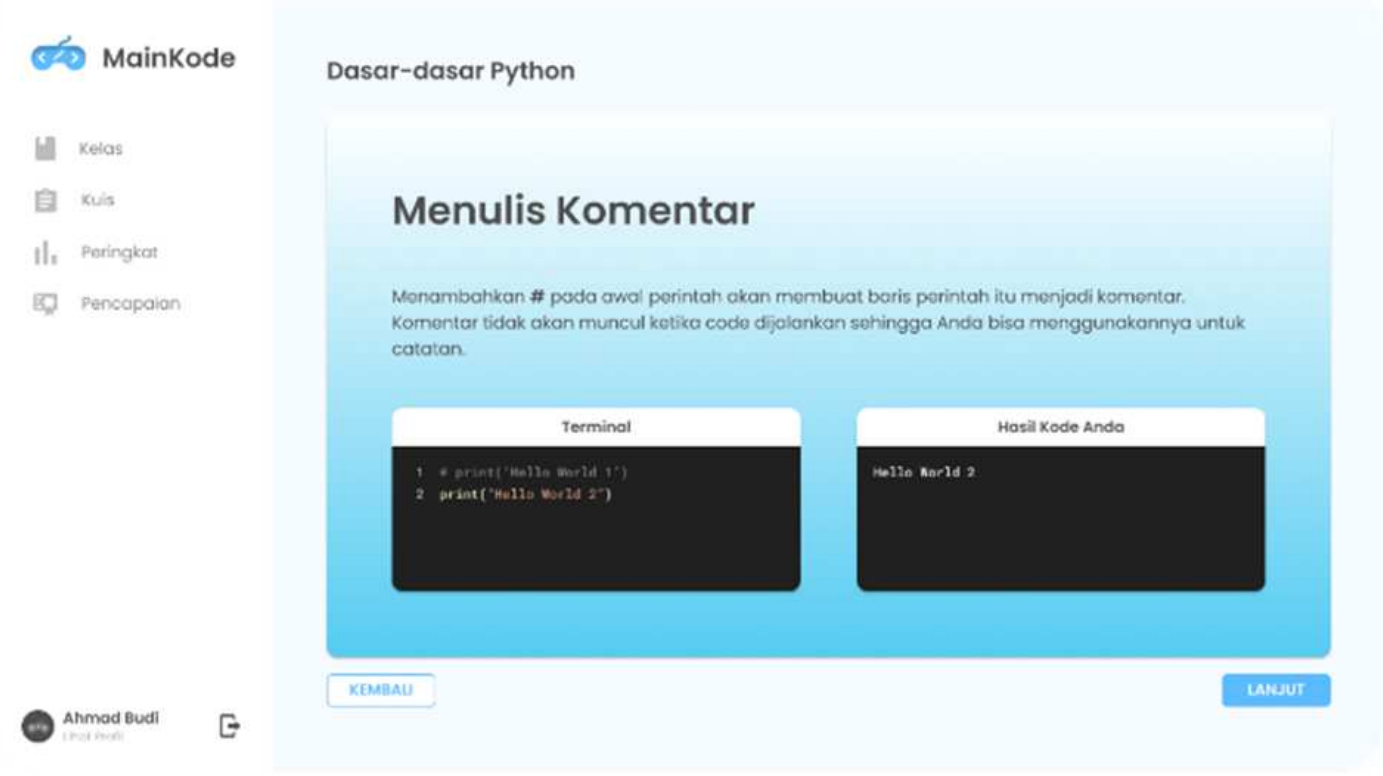
\includegraphics[width=\linewidth]{contents/chapter-2/images/Evan-a1.png}
	  \caption{\textit{Class topic page}}
	  \label{fig:sub1-a1}
	\end{subfigure}
	\begin{subfigure}[b]{0.4\textwidth}
	\centering
	  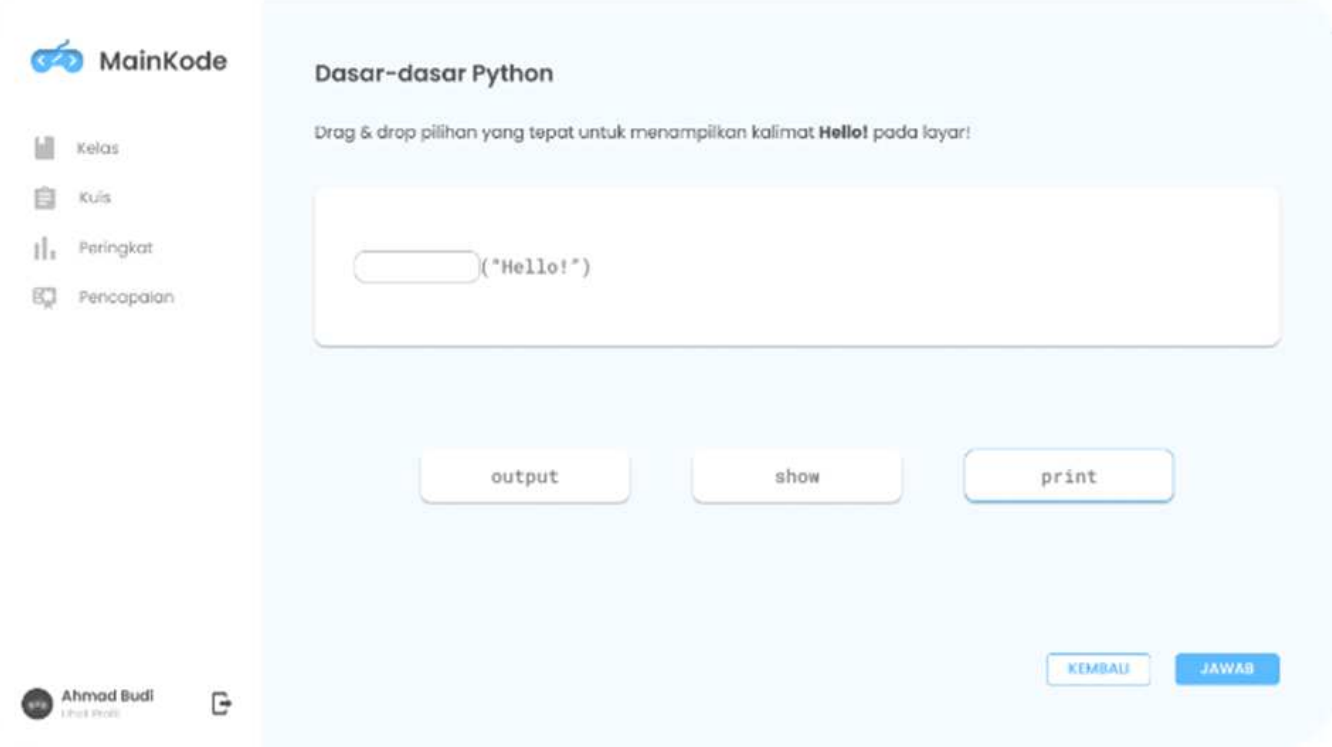
\includegraphics[width=\linewidth]{contents/chapter-2/images/Evan-a2.png}
	  \caption{\textit{Gamified exercise page}}
	  \label{fig:sub2-a2}
	\end{subfigure}
	\hfill
	\begin{subfigure}[b]{0.4\textwidth}
		\centering
		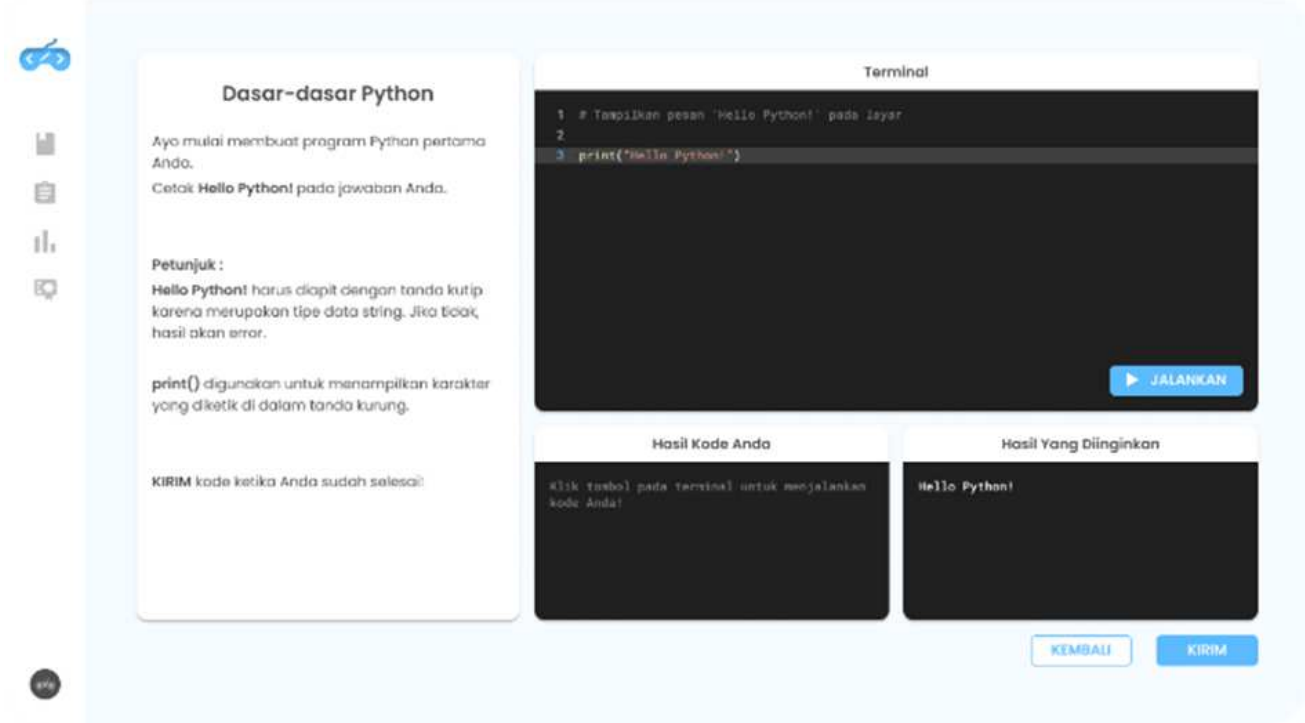
\includegraphics[width=\linewidth]{contents/chapter-2/images/Evan-a3.png}
		\caption{\textit{Terminal exercise page}}
		\label{fig:sub3-a3}
	\end{subfigure}  
	\begin{subfigure}[b]{0.4\textwidth}
		\centering
		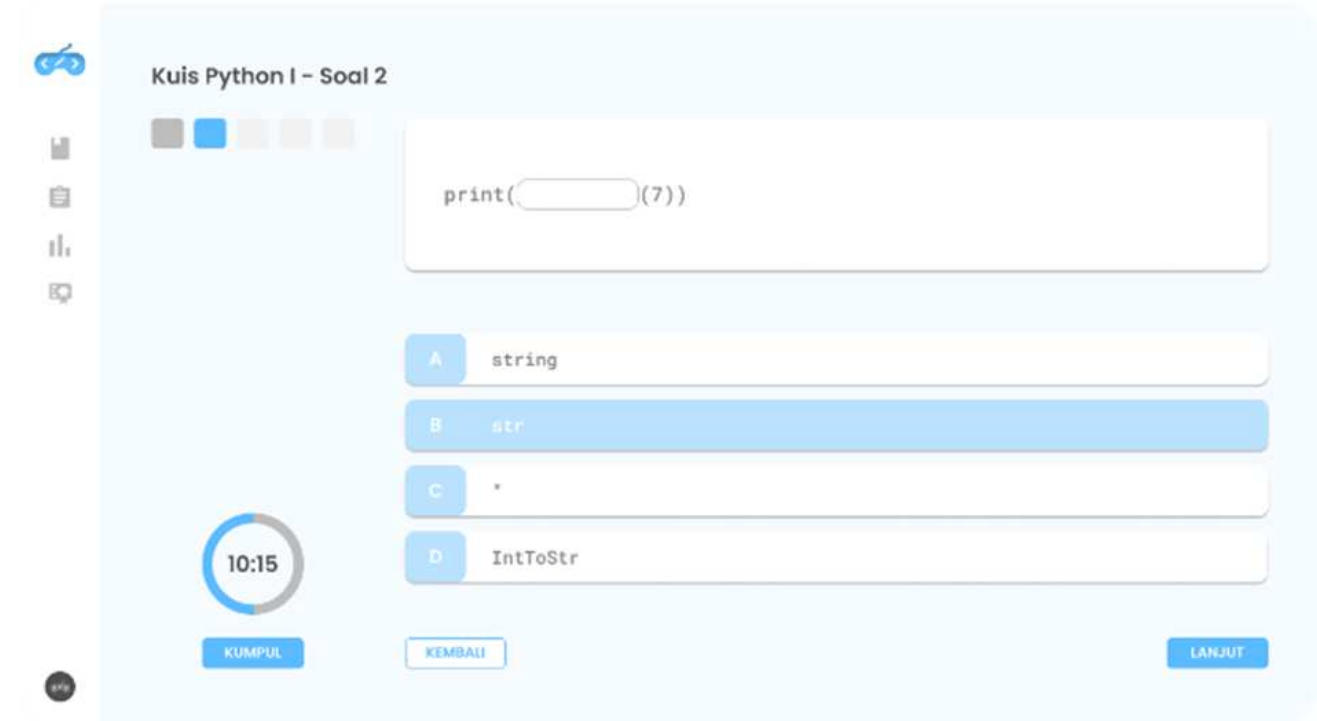
\includegraphics[width=\linewidth]{contents/chapter-2/images/Evan-a4.png}
		\caption{\textit{Quiz page}}
		\label{fig:sub4-a4}
	\end{subfigure} 
	\begin{subfigure}[b]{0.4\textwidth}
		\centering
		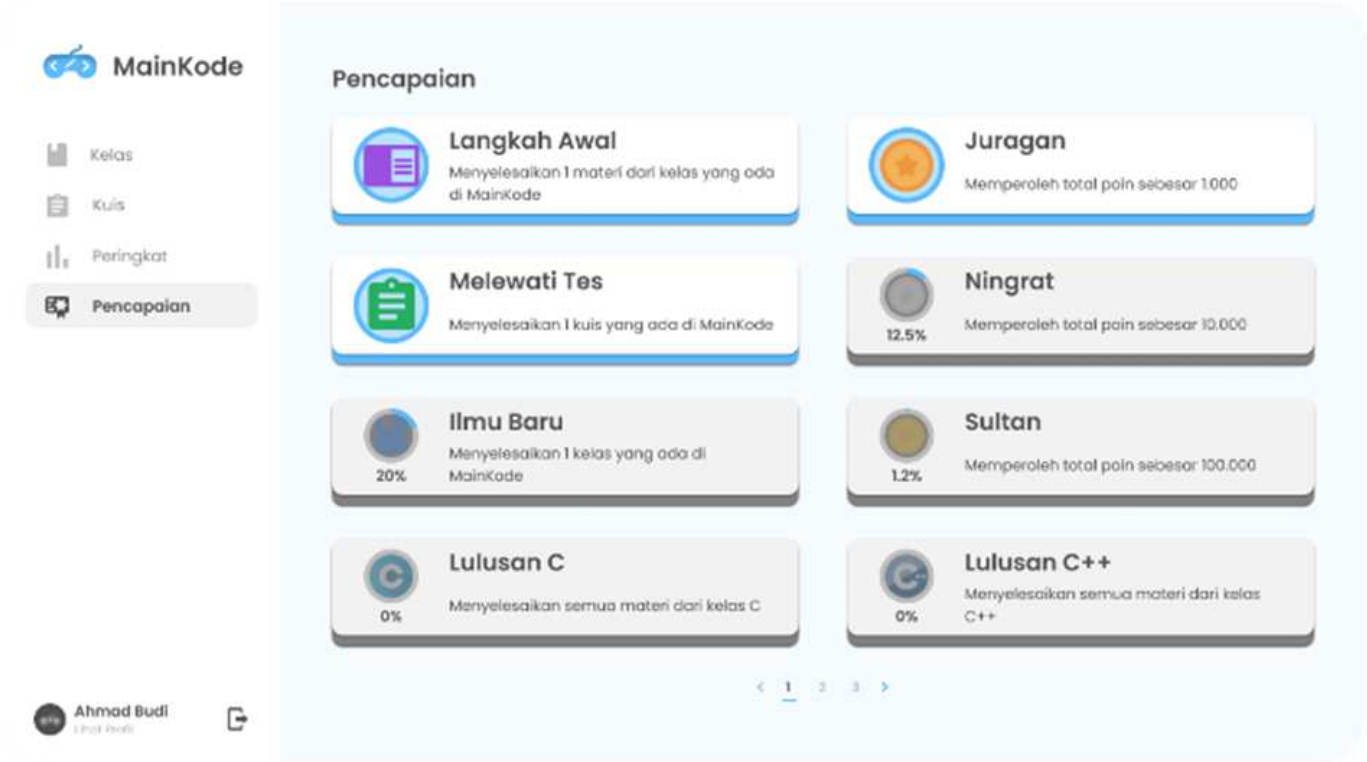
\includegraphics[width=\linewidth]{contents/chapter-2/images/Evan-a5.png}
		\caption{\textit{Achievement page}}
		\label{fig:sub5-a5}
	\end{subfigure} 
	\caption{\textit{High-fidelity prototype} aplikasi pembelajaran pemrograman}
	\label{fig:High-fidelity prototype Evan}
  \end{figure}
% ================================= Penelitian Design of Gamification for Anatomy Learning Media =================================
Ada juga penelitian yang dilakukan pada tahun 2021 oleh Bernadeta Ratna P. S. dan rekan-rekannya mengenai pengembangan desain gamifikasi ini.
Penelitian tersebut memaparkan mengenai pengembangan gamifikasi untuk sebuah media pembelajaran anatomi yang berjudul \textit{"Design of Gamification for Anatomy Learning Media"}.
Sama halnya dengan penelitian sebelumnya, penelitian ini memiliki tujuan untuk meningkatkan motivasi dan keterlibatan pengguna dalam memahami anatomi tubuh manusia.
Proses pengembangan desain gamifikasi pada penelitian ini menggunakan sebuah \textit{framework game design} yang dinamai \textit{"Elemental Tetrad"}.
\textit{Framework} memodelkan gamifikasi dalam 4 bentuk, yakni \textit{Mechanics},\textit{Aesthetics}, \textit{Story} atau \textit{Dynamics}, dan \textit{Technology}.
Masing masing elemen desain tersebut kemudian dikembangkan berdasarkan konteks pembelajaran yang akan dipelajari, dalam penelitian ini yaitu pembelajaran anatomi manusia.
\textit{Game Mechanics} dalam penelitiannya terdiri dari \textit{game mode}, \textit{parts}, \textit{points} dan\textit{reward}. 
Untuk elemen \textit{Aesthetics} terdiri dari \textit{ User Interface dan User Experience}, \textit{Art}, \textit{Unlocking Parts}, dan \textit{Challenges}.
Untuk \textit{Story}, akan mengikuti alur pembelajaran yang dibagi menjadi 3 bagian, yaitu materi, praktikum, dan kuis.
Untuk elemen terakhir yaitu teknologi yang digunakan dalam penelitian ini. Penelitian ini menggunakan \textit{Smartphone} dan 3D model dari kerangka manusia.
% \newpage
\begin{figure}[htbp]
	\centering
	\begin{subfigure}[b]{0.4\textwidth}
		\centering
	  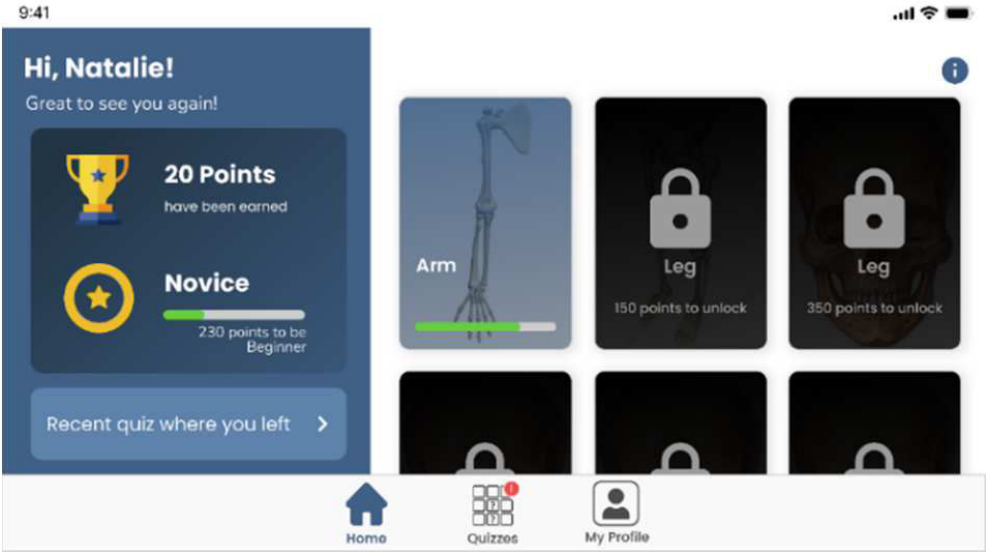
\includegraphics[width=\linewidth]{contents/chapter-2/images/Deta-a1.png}
	  \caption{\textit{Interface design home menu}}
	  \label{fig:sub-deta-a1}
	\end{subfigure}
	\begin{subfigure}[b]{0.4\textwidth}
	\centering
	  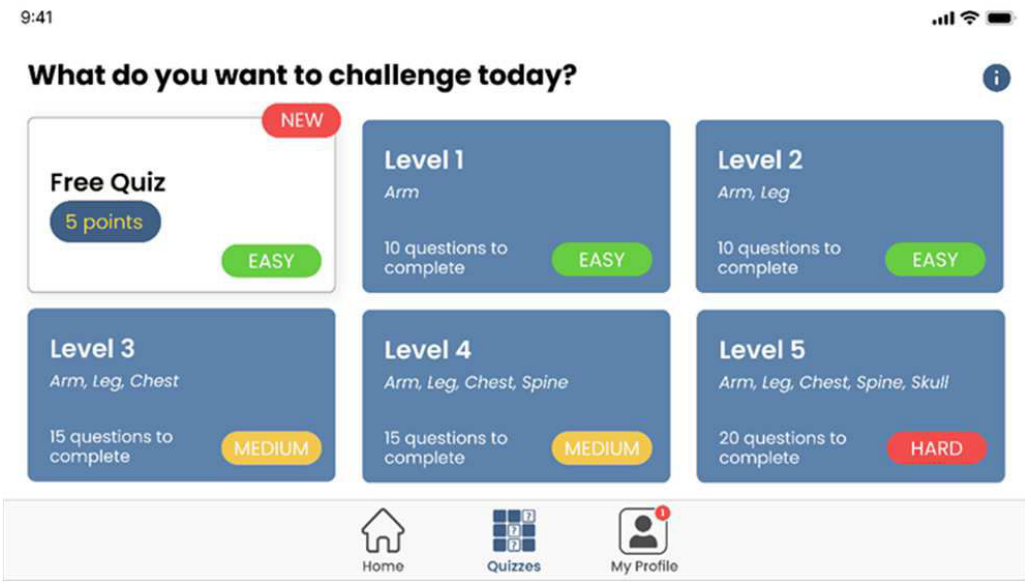
\includegraphics[width=\linewidth]{contents/chapter-2/images/Deta-a2.png}
	  \caption{\textit{Interface design quiz menu }}
	  \label{fig:sub-deta-a2}
	\end{subfigure}
	\hfill
	\begin{subfigure}[b]{0.4\textwidth}
		\centering
		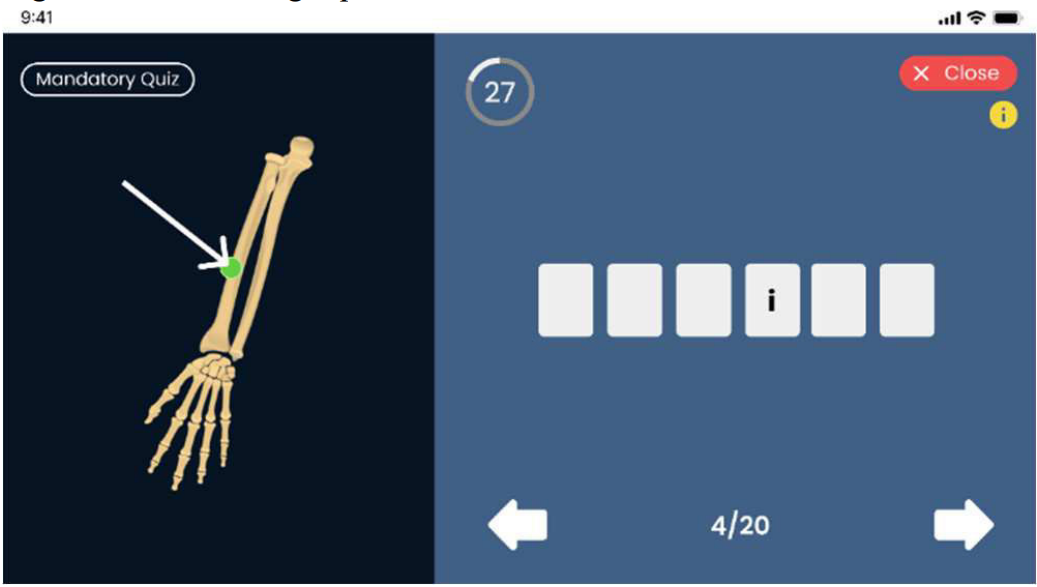
\includegraphics[width=\linewidth]{contents/chapter-2/images/Deta-a3.png}
		\caption{\textit{Interface design mandatory quiz}}
		\label{fig:sub-deta-a3}
	\end{subfigure}  
	\caption{Tampilam aplikasi pembelajaran anatomi}
	\label{fig:interface pembelajaran anatomi}
  \end{figure}
Hasil dari penelitianini berupa sebuah aplikasi \textit{Smartphone} yang dapat diinstall pada sistem operasi Android.
Tampilan aplikasi ini dilampirkan pada gamabar \ref*{fig:interface pembelajaran anatomi}.
Berbeda dengan penelitian sebelumnya, pada penelitian ini tidak dilakukan pengujian \textit{Usability} dan \textit{User Experience}.

Pengadaptasian gamifikasi pada sebuah media pembelajaran juga dijelasakan pada penelitian yang dilakukan oleh Andre Julian Irawan, Fenina Adline Twince Tobing, dan Eunike Endariahna Surbakti
dengan judul \textit{"Implementation of Gamification Octalysis Method at Design and Build a React Native Framework Learning Application"}.
Dalam penelitian ini, proses gamifikasi menggunakan kerangka kerja \textit{Octalysis} atau \textit{Octalysis Gamification Framework} untuk mengembangan sebuah aplikasi pembelajaran yang mempelajari \textit{React Native Framework}.
Kerangka kerja ini meruapakan sebuah kerangka kerja gamifikasi yang dikembangakan oleh Yu-Kai Chou, seorang ahli gamifikasi terkemuka[].
Metode \textit{Octalysis} memiliki delapan inti motivasi yang berfokus pada perilaku manusia, seperti \textit{meaning}, \textit{accomplishment}, \textit{empowerment}, \textit{ownership}, \textit{social influence}, \textit{scarcity}, \textit{unpredictability}, dan \textit{avoidance}.
Untuk mengukur keberhasilan dari penerapan gamifikasi yang dilakukan, penelitian ini mengerjakan beberapa pengujian untuk aplikasi yang dikembangkan.
Penelitian ini menggunakan \textit{Hedonic Motivation System Adoption Model (HMSAM)} untuk mengukur motivasi intrinsik dari sebuah sistem atau aplikasi.
Selain itu juga, dalam penelitian ini dialkukan pengukuran sikap, pendapat, dan persepsi seseorang tentang fenomena sosial dengan skala Likert atau \textit{Likert Scale}.
\newpage
\begin{figure}[htbp]
	\centering
	\begin{subfigure}[b]{0.4\textwidth}
		\centering
	  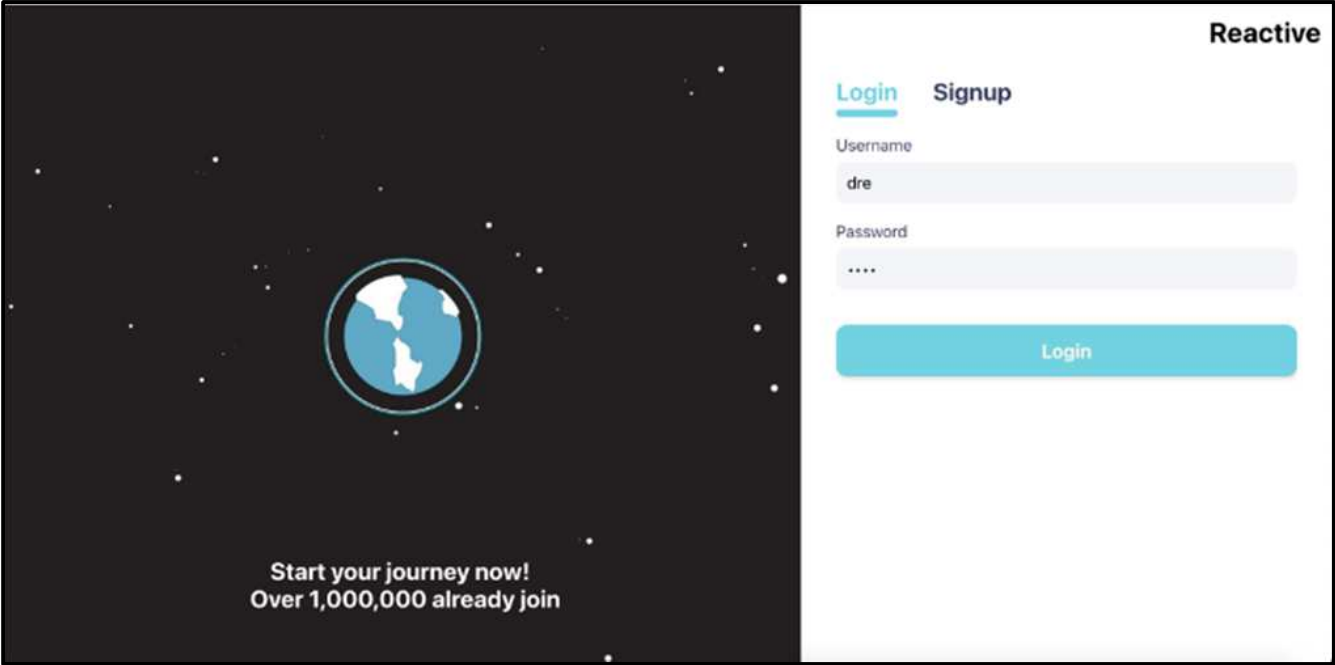
\includegraphics[width=\linewidth]{contents/chapter-2/images/Andre-a1.png}
	  \caption{\textit{Interface design home menu}}
	  \label{fig:sub-andre-a1}
	\end{subfigure}
	\begin{subfigure}[b]{0.4\textwidth}
	\centering
	  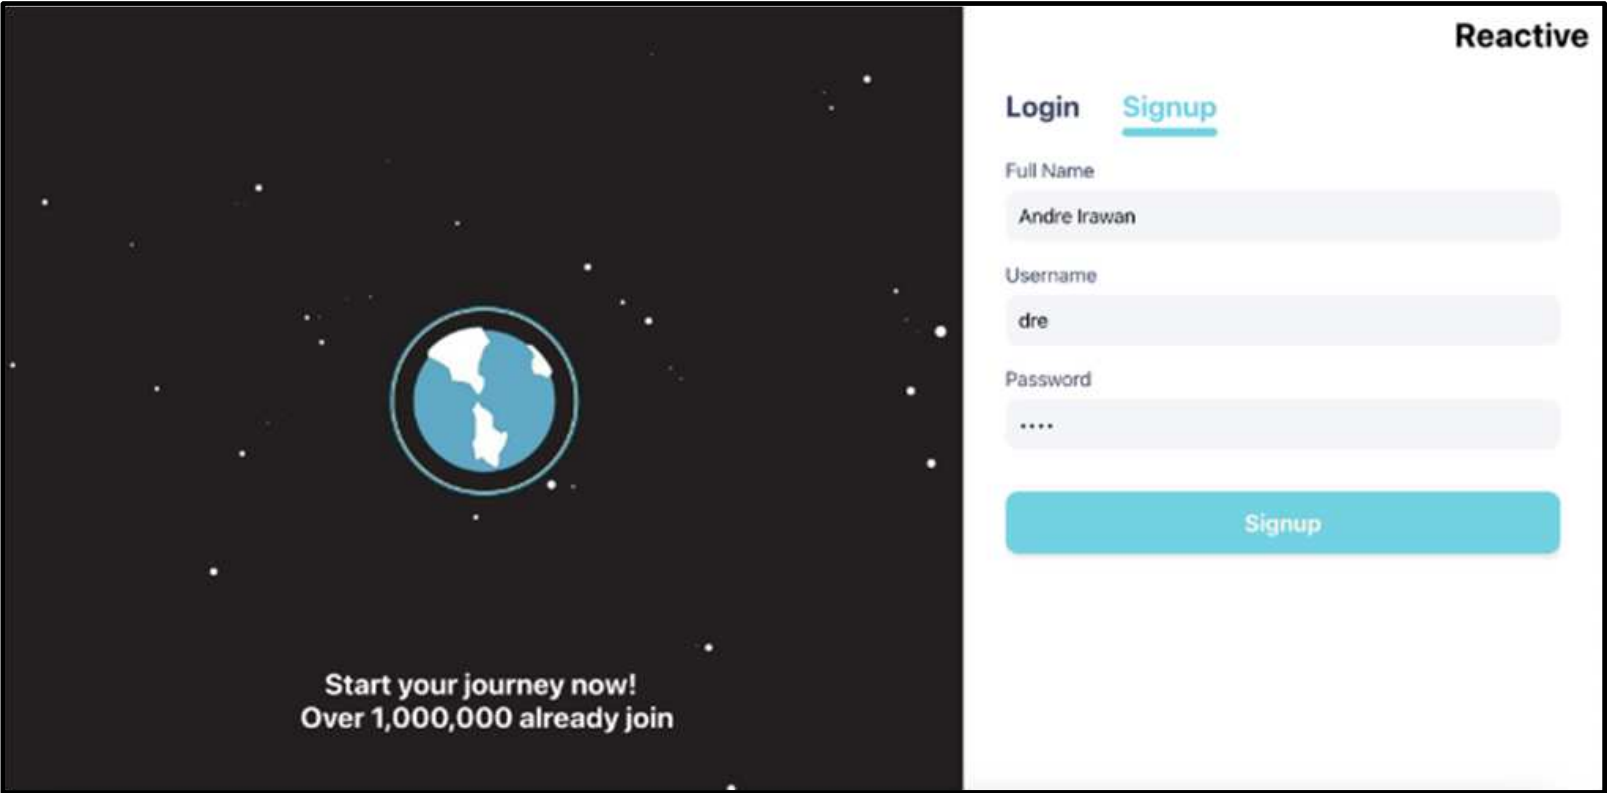
\includegraphics[width=\linewidth]{contents/chapter-2/images/Andre-a2.png}
	  \caption{\textit{Interface design quiz menu }}
	  \label{fig:sub-andre-a2}
	\end{subfigure}
	\hfill
	\begin{subfigure}[b]{0.4\textwidth}
		\centering
		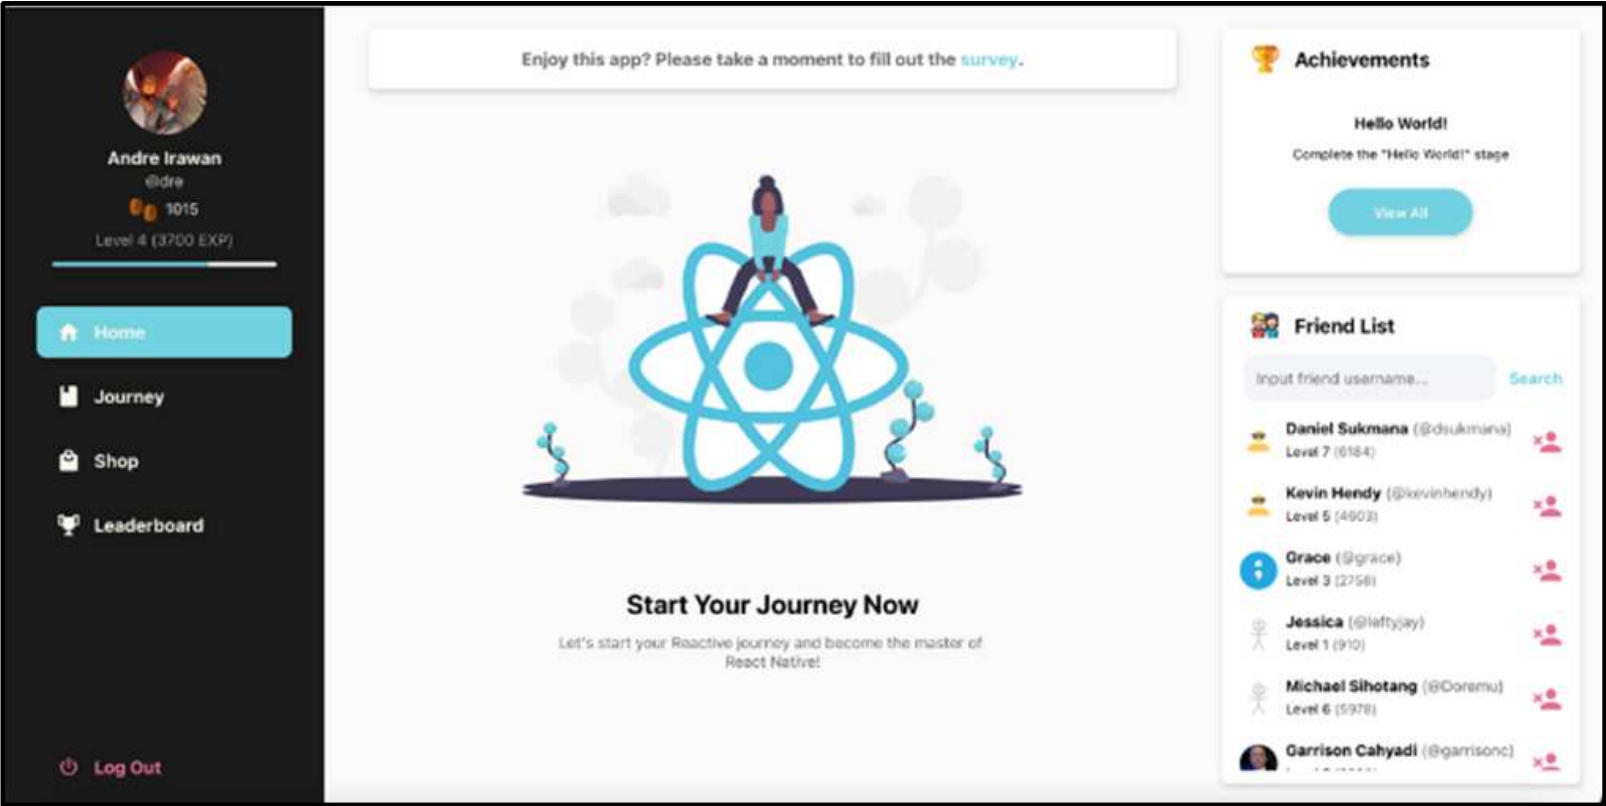
\includegraphics[width=\linewidth]{contents/chapter-2/images/Andre-a3.png}
		\caption{\textit{Interface design mandatory quiz}}
		\label{fig:sub-andre-a3}
	\end{subfigure}  
	\caption{Tampilam aplikasi pembelajaran \textit{React Native App}}
	\label{fig:interface pembelajaran React Native}
\end{figure}
\section{Analisis Perbandingan Metode}
Dari tinjauan pustaka yang dilakukan oleh penulis, penulis menemukan perbedaan metode desain dan pengembangan gamifikasi yang dugunakan pada setiap penelitian.
Perbedaan ini didasari dengan konteks pembelajaran yang akan dikembangkan, dan bagaimana aplikasi pembelajaran didesain dan dikembangkan.
Faktor lain perbedaan metode ini juga didasari oleh kebutuhan pengguna dan target device dimana aplikasi tersebut akan berjalan.
Penelitian yang dilakukan oleh Evan dan rekan-rekannya menggunakan metode \textit{Activity-centered Design} dimana metode ini dipilih karena aplikasi ini akan berfokus pada aktifitas utama pemrograman.
Berbeda halnya dengan penelitian yang dilakukan oleh Bernadeta dan rekan-rekan rekannya. Metode pengembangan aplikasi ini didasari dengan framework gamifikasi yang sudah ada sebelumnya yaitu \textit{Elemental Tetrad}.
Penelitian ini mendesain sebuah gamifikasi pembelajaran anatomi berdasarkan setiap elemen yang ada di \textit{Elemental Tetrad Framework}.
Penelitian yang dilakukan oleh Julian dan teman-temannya memiliki metode desain yang sama menggunakan sebuah kerangka kerja gamifikasi, 
bedanya  pada penelitiannya tersebut mereka menggunakan \textit{Octalysis} sebagai kerangka kerjanya. \textit{Framework} ini menggunakan 8 elemen yang fokus pada kebiasaan manusia.
Perbedaan antara kedua \textit{Framework} gamifikasi tersebut adalah dari tujuan kerangka kerjanya. Kerangka kerja \textit{Elemental Tetrad} berfokus pada pembentukan pengalaman Gamifikasi,
sedangkan \textit{Octalysis} berfokus pada pengaruh motivasi dan keterlibatan pengguna dalam gamifikasi.
% Metode tersebut dapat divisualisasikan dengan gambar \ref*{Fig:itterative-Design Cycle}
% \begin{figure}[H]
% 	\centering
% 	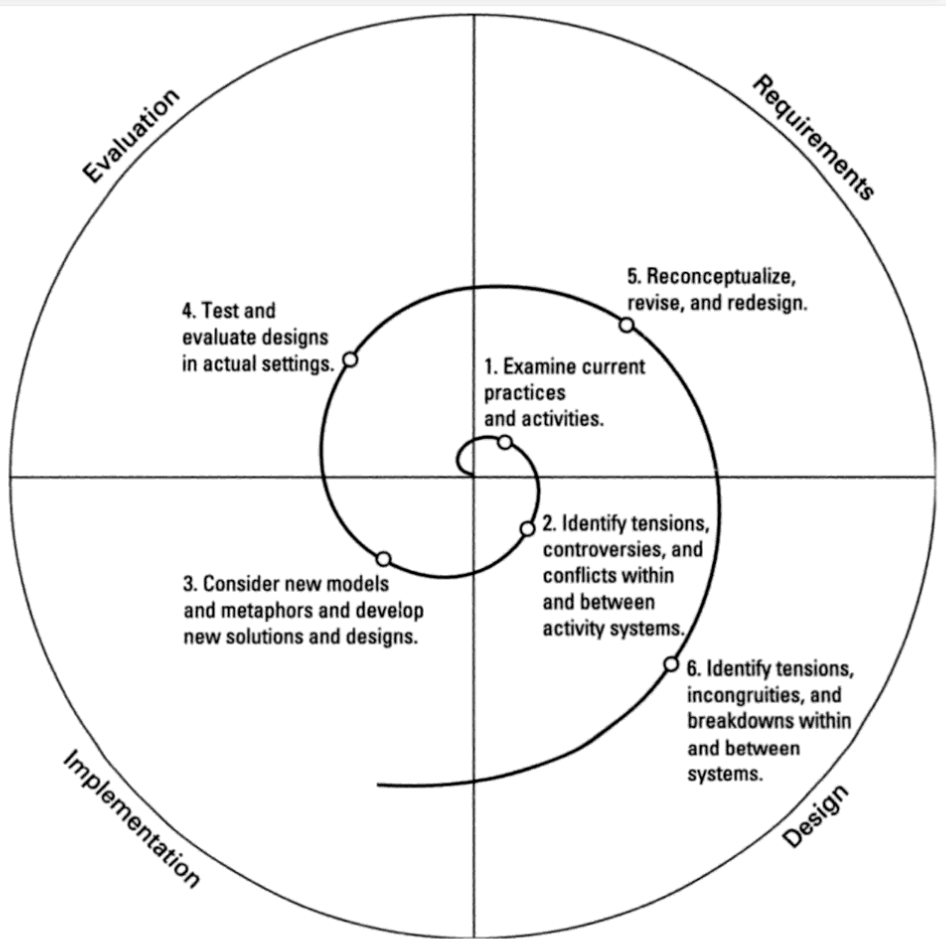
\includegraphics[width=6cm]{contents/chapter-2/images/Itterative-design.png}
% 	\caption[Caption]{An itterative-Design Cycle \cite{2004activity}}
% 	\label{Fig:itterative-Design Cycle}
% \end{figure}
\newpage
\begin{landscape}
	\begin{table}[htbp]
	\caption{Perbandingan Penelitian}
	\centering
	\begin{tabular}{|>{\centering\arraybackslash}m{0.5cm}|m{4cm}|m{3.5cm}|m{4.5cm}|m{4.5cm}|m{4cm}|m{4cm}|}
		\hline
		\centering \textbf{No} & \centering \textbf{Judul Penelitian} & \centering \textbf{Penulis} & \centering  \textbf{Pengembangan Desain Gamifikasi} &\centering\textbf{Fokus}&\multicolumn{1}{m{4cm}|}{\centering\textbf{Luaran}} \\
		\hline 
		1 & Designing Gamification for Programming Learning Applications 
		& 
		Evan Pradanika, Yani Widyani,  Yanti Rusmawati
		& Activity-centered Design \& Type of Knowledge and Gamification Element Relation& Merancang pengalaman pengguna yang optimal dengan memahami kebutuhan, konteks, dan tujuan aktivitas& High-fidelity Prototype Aplikasi\\
		\hline
		2 & Design of Gamification for Anatomy Learning Media 
		& 
		Adhistya Erna Permanasari, Bernadeta Ratna P S, Fikry Yanuar S, Mirza Putri Maharani, Sunu Wibirama, Junaedy Yunus
		& Elemental Tetrad Gamification Framework& Membentuk pengalaman gamifikasi & Aplikasi Mobile\\
		\hline
		3 & 
		Implementation of Gamification Octalysis Method at Design and Build a React Native Framework Learning Application 
		& 
		Andre Julian Irawan, Fenina Adline Twince Tobing, Eunike Endariahna Surbakti
		& Octalysis Gamification Framework& Mempengaruhi Motivasi dan Keterlibatan pengguna & Aplikasi Web React Native\\
		\hline
	  \end{tabular}
	\end{table}
	% \begin{table}
	% 	\caption{Perbandingan Penelitian}
	% 	\centering
	% 	\begin{tabular}{|>{\centering\arraybackslash}m{1cm}|m{5cm}|m{5cm}|m{5cm}|m{5cm}|m{5cm}|}
	% 		\hline
	% 		\centering No & \centering Judul Penelitian & \centering Penulis & \centering  Pengembangan Desain Gamifikasi &\multicolumn{1}{m{5cm}|}{\centering\textbf{Examples}} \\
	% 		\hline 
	% 	  \end{tabular}
	% 	\end{table}
\end{landscape}

\newpage
\section{Dasar Teori}
\subsection{Media Pembelajaran}
\subsection{Teori Game}
\subsubsection{Elemental Tetrad} 
Elemental Tetrad adalah sebuah kerangka konseptual yang digunakan dalam desain dan analisis produk atau layanan digital. 
Konsep ini pertama kali diperkenalkan oleh Jesse James Garrett, seorang desainer pengalaman pengguna terkemuka, 
dan berfokus pada empat elemen utama yang saling berinteraksi dalam pengalaman pengguna digital.

\subsubsection{The MDA Framework}
MDA (Mechanics, Dynamics, Aesthetics) Framework adalah sebuah kerangka kerja yang digunakan dalam pengembangan permainan
(game development) untuk menganalisis dan memahami elemen-elemen inti yang membentuk pengalaman bermain game. 
Konsep ini pertama kali diperkenalkan oleh Robin Hunicke, Marc LeBlanc, dan Robert Zubek pada tahun 2004.
\subsubsection{The Game Design Spiral}
Game Design Spiral (lingkaran desain permainan) adalah pendekatan iteratif 
dalam desain permainan yang menggabungkan siklus pengembangan dan pengujian berulang untuk menciptakan 
permainan yang lebih baik seiring berjalannya waktu. Pendekatan ini memungkinkan desainer permainan untuk 
memperbaiki dan meningkatkan desain mereka melalui siklus yang terus berulang.
\subsection{Gamifikasi}
\subsection{FDD}
\subsection{Black Box Testing}
\subsection{\textit{System Usability Testing}(SUS)}
\subsection{\textit{User Experience Questionnaire}(UEQ)}


% Di dalam tinjauan pustaka hasil akhirnya adalah analisis secara kualitatif atau pun secara kuantitatif kelebihan dan kekurangan metode jika dikaitkan dengan masalah, batasan-batasan masalah dan solusi yang dinginkan.
% Analisis kuantitatif tidak wajib teapi mempunyai nilai tambah di dalam tugas akhir saudara. Bagian ini menjelaskan kenapa metode tersebut dipilih dan uraikan dengan lebih jelas metode pelaksanaan tugas akhir yang ingin Anda lakukan. 
% \section{Pertanyaan Tugas Akhir (Jika Perlu)}

% Pertanyaan tugas akhir bersifat opsional dan dapat ditambahkan untuk menekankan hal-hal yang hendak diketahui dari tugas akhir berdasar pada tujuan tugas akhir. Pertanyaan tugas akhir dikenal dengan RQ (\textit{Research Question}) dan harus memiliki keterkaitan dengan RO (\textit{Research Objective}). Satu RO dapat memiliki satu atau lebih dari satu RQ. 


\chapter{Metode Penelitian}
Pada bab ini, akan dilakukan penjelasan mengenai alat dan bahan pendukung dari tugas akhir ini.
Alat dan bahan tersebut berupa perangkat keras, perangkat lunak, dan bahan data.
Selain itu, bab ini juga akan memaparkan mengenai alur dan urutan pengerjaan Tugas Akhir.
\section{Alat dan Bahan Tugas akhir}
Alat yang digunakan untuk mengembangkan Aplikasi ini terdiri dari Perangkat Keras dan Perangkat Lunak.
\subsection{Alat Tugas akhir}
\subsubsection{Perangkat Keras}
\begin{enumerate}
	\item \textit{laptop} dengan spesifikasi minimum anu, 
	pada tugas akhir ini digunakan \textit{Laptop Asus ROG Zephyrus G14} dengan spesifikasi sistem operasi Windows 11, \textit{processor} AMD Ryzen 5 4600HS with Radeon Graphics @ 3,00 GHz, memori 16GB DDR4, grafis NVIDIA GeForce GTX 1650Ti (4GB), SSD 512GB.
	\item \textit{Smartphone} dengan spesifikasi minimum anu, pada tugas akhir ini digunakan \textit{Smartphone Samsung Galaxy S20 Ultra} dengan spesifikasi OS Android 13 (Tiramisu), CPU Octa-core (2x2.73 GHz Mongoose M5, 2x2.50 GHz Cortex-A76, 4x2.0 GHz Cortex-A55), GPU Mali-G77 MP11, Internal 128 GB, 12GB RAM.
\end{enumerate}

\subsubsection{Perangkat Lunak}
\begin{enumerate}
	\item \textit{laptop} dengan spesifikasi minimum anu, 
	pada tugas akhir ini digunakan \textit{Laptop Asus ROG Zephyrus G14} dengan spesifikasi sistem operasi Windows 11, \textit{processor} AMD Ryzen 5 4600HS with Radeon Graphics @ 3,00 GHz, memori 16GB DDR4, grafis NVIDIA GeForce GTX 1650Ti (4GB), SSD 512GB.
	\item \textit{Smartphone} dengan spesifikasi minimum anu, pada tugas akhir ini digunakan \textit{Smartphone Samsung Galaxy S20 Ultra} dengan spesifikasi OS Android 13 (Tiramisu), CPU Octa-core (2x2.73 GHz Mongoose M5, 2x2.50 GHz Cortex-A76, 4x2.0 GHz Cortex-A55), GPU Mali-G77 MP11, Internal 128 GB, 12GB RAM.
\end{enumerate}
% \begin{enumerate}
% 	\item Microsoft Visual Studio Code 2022
% 	\item Figma
% \end{enumerate}
\newpage
\subsection{Bahan Tugas akhir}
Bahan yang digunakan untuk Tugas Akhir ini ialah sebagi berikut :
\begin{enumerate}
	\item Materi mata kuliah \textit{System Diagnosis Berbasis Pembantu Keputusan} (SBPK) dari Departemen Teknik Elektro dan Teknologi Informasi berupa file .pptx
	\item Data hasil wawancara pada Mahasiswa Teknik Biomedis yang telah memperolah mata kuliah SDBPK untuk kebutuhan \textit{User Persona}
\end{enumerate}
% \begin{itemize}
% 	\item Dataset pihak lain yang diperoleh dengan izin atau dalam lisensi yang diizinkan untuk digunakan secara langsung 
% 	\item Dataset pihak pertama yang disusun sendiri melalui quisioner, observasi, atau interview 
% 	\item Dokumen panduan yang mengacu pada standar, hasil tugas akhir, atau artikel yang disitasi dan digunakan.
% \end{itemize}


\section{Metode yang Digunakan}

Metode yang akan dipakai dalam tugas akhir akan dibagi menjadi Pengembangan Aplikasi, Pengembangan Desain Aplikasi, serta Pengujian Aplikasi dan Efektifitas Aplikasi.
Untuk pengembangan Aplikasi pada Tugas Akhir ini akan diterapkan metode FDD atau \textit{Feature-Driven Development}, metode ini digunakan karena

Untuk Pengembangan Design Gamifikasi pada tugas akhir ini akan diterapkan metode pengembangan.....

Untuk pengujiannya sendiri, aplikasi ini akan diuji dengan Black Box testing untuk menguji Fitur fitur.....



\section{Alur Tugas Akhir}

Tugas Akhir ini akan dibagi menjadi tahap \textit{Development} dan Tahap pengujian.
Untuk tahap \textit{Development} sendiri akan menggunakan metode \textit{Feature-Driven Development} untuk mengembangkan Softwarenya.
Proses \textit{Development} ini termasuk juga proses perancangan Gamifikasi yang akan diadopsi pada Aplikasi.
Untuk tahap pegujian, penulis akan mengujikan Fungsionalitas Aplikasi yang telah dikembangkan menggunakan Pengujian \textit{Black Box Testing}.
Kemudian dilanjutkan dengan Pengujian \textit{System Usability Scale} dan \textit{User Experience Questionnaire} untuk mengevaluasi pengalamaan pengguna mengenai Aplikasi yang telah dikembangkan.
Secara keseluruhan, Alur Tugas Akhir ini dapat dilihat pada gambar \ref{Fig:Alur Tugas Akhir}
\begin{figure}[H]
	\centering
	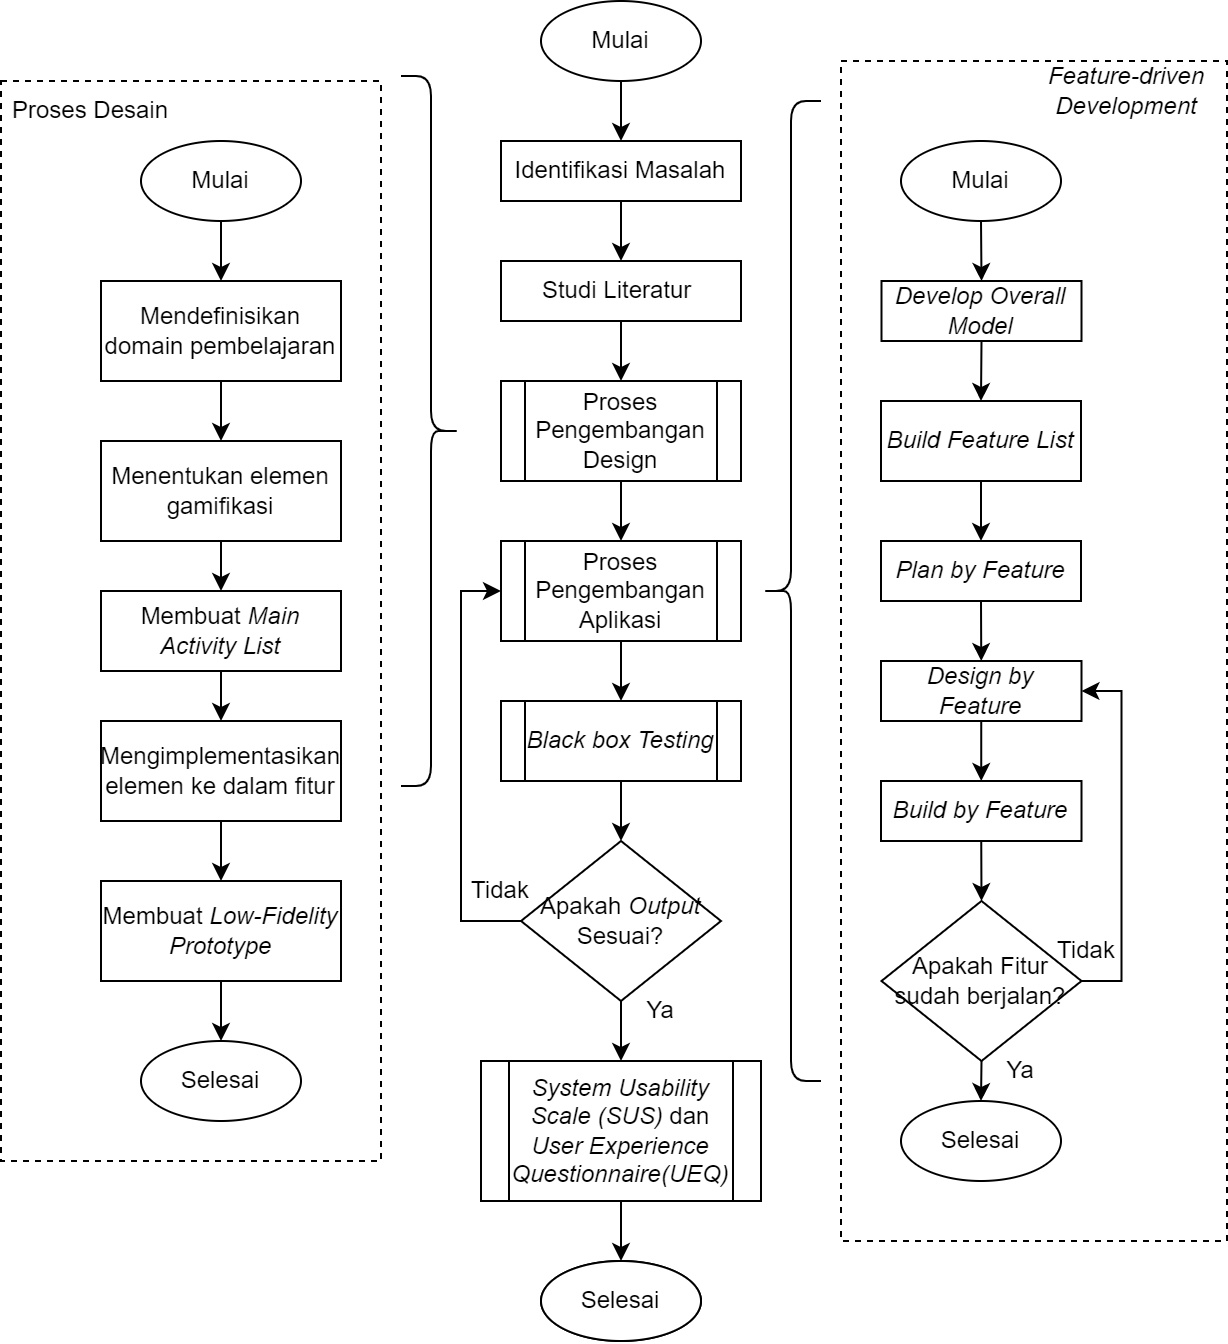
\includegraphics[width=12cm]{contents/chapter-3/images/Alur-tugas-akhir.png}
	\caption[Caption]{Alur Tugas Akhir}
	\label{Fig:Alur Tugas Akhir}
\end{figure}
% \section{Etika, Masalah, dan Keterbatasan Penelitian (Opsional)}
\subsection{Identifikasi Masalah}
\subsection{Studi Literatur}
\subsection{Observasi dan memperlajari Aplikasi dengan Gamifikasi}
\subsection{\textit{Develop Overall Model}}
\subsection{\textit{Build Feature List}}
% \subsection(\textit{Designing GAmification Based on Feature})
\subsection{\textit{Plan by Feature}}
\subsection{\textit{Design by Feature}}
\subsection{\textit{Build by Feature}}
\subsection{Menguji Fungsionalitas Aplikasi \textit{Black Box Testing}}
\subsection{Pengujian Aplikasi}

% Bagian ini membahas pertimbangan etis penelitian dan [potensi] masalah serta
% keterbatasannya. Jika menyangkut penelitian dengan makhluk hidup, maka dibutuhkan adanya \textit{ethical clearance}, di bagian ini hal itu akan dibahas. Demikian juga tentang keterbatasan ataupun masalah yang akan timbul.

\chapter{Hasil dan Pembahasan}

\section{Desain Gamifikasi}

Poin pertama adalah membahas tujuan penelitian pertama. 
Dapat ditambahkan beberapa sub bab jika diperlukan.

\section{Aplikasi}

Poin kedua adalah membahas tujuan penelitian kedua. Dapat ditambahkan beberapa 
sub bab jika diperlukan. Dapat juga diteruskan ke Sub Bab Pembahasan hasil 3 dan 
seterusnya, jika ada tiga atau lebih tujuan penelitian.

\section{Analisis Hasil Pengujian}

Pembahasan penutup dapat menjelaskan mengenai kelebihan hasil pengembangan / 
penelitian dan kekurangan dibandingkan dengan skripsi atau penelitian terdahulu atau
perbandingan terhadap produk lain yang ada di pasaran. Penulis dapat menggunakan tabel untuk membandingkan secara gamblang dan menjelaskannya.
\chapter{Kesimpulan dan Saran}

\section{Kesimpulan}

Kesimpulan dapat diawali dengan apa yang dilakukan dengan tugas akhir ini lalu 
dilanjutkan dengan poin-poin yang menjawab tujuan penelitian, apakah tujuan sudah tercapai atau belum, tentunya berdasarkan data ataupun hasil dari Bab pembahasan sebelumnya. Dalam beberapa hal, kesimpulan dapat juga berisi tentang temuan/\textit{findings} yang Anda dapatkan setelah melakukan pengamatan dan atau analisis terhadap hasil penelitian. 

\section{Saran}

Saran berisi hal-hal yang bisa dilanjutkan dari penelitian atau skripsi ini, yang belum dilakukan karena batasan permasalahan. Saran bukan berisi saran kepada sistem atau pengguna, tetapi saran diberikan kepada aspek penelitian yang dapat dikembangkan dan ditambahkan di penelitian atau skripsi selanjutnya.

% \chapter{Kesimpulan dan Saran}

\section{Kesimpulan}

Kesimpulan dapat diawali dengan apa yang dilakukan dengan tugas akhir ini lalu 
dilanjutkan dengan poin-poin yang menjawab tujuan penelitian, apakah tujuan sudah tercapai atau belum, tentunya berdasarkan data ataupun hasil dari Bab pembahasan sebelumnya. Dalam beberapa hal, kesimpulan dapat juga berisi tentang temuan/\textit{findings} yang Anda dapatkan setelah melakukan pengamatan dan atau analisis terhadap hasil penelitian. 

\section{Saran}

Saran berisi hal-hal yang bisa dilanjutkan dari penelitian atau skripsi ini, yang belum dilakukan karena batasan permasalahan. Saran bukan berisi saran kepada sistem atau pengguna, tetapi saran diberikan kepada aspek penelitian yang dapat dikembangkan dan ditambahkan di penelitian atau skripsi selanjutnya.


%======================================

%======================================
%  References
%======================================
\thereferences
% You can change 
%    the filename and location of the files inputted
\bibliography{references}


%======================================

%======================================
%  Appendix
%======================================
% You can change 
%    the filename and location of the files inputted
%    use \chapterappendix for the first page of the appendix
%    use \chapterappendixadd for the next page

\appendix


\chapterappendix{contents/appendix/appendix-isi-lampiran}
\chapterappendixadd{contents/appendix/appendix-latex}
\chapterappendixadd{contents/appendix/appendix-penulisan-referensi}
\chapterappendixadd{contents/appendix/appendix-code}




%======================================

\end{document}